\documentclass[10pt, nofootinbib, twocolumn]{revtex4-1}
\usepackage{amsmath}
\usepackage{xparse}
\usepackage{graphicx}
\usepackage{hyperref}
\usepackage{color}
\usepackage{physics}
\usepackage{enumitem}
\usepackage{natbib}
\usepackage{booktabs}
\usepackage{float}
\usepackage{caption}
\usepackage{mathtools}
\usepackage{multirow}

\hypersetup{
    colorlinks=true,
    linkcolor=black,  
    citecolor=black,
    urlcolor=blue
}

\begin{document}
\vspace*{2\baselineskip}
\title{Project1 AST3310 - Modelling Stellar Engines} 
\vspace*{3\baselineskip}
\date{\today} \homepage{https://github.com/tirilsg/AST3310_Project1}       
\begin{abstract}
\vspace*{1\baselineskip}
\textit{A model for energy production within a stellar core based on the behaviour observed within the sun is implemented in this report. A python class taking temperature and stellar core density as arguments is implemented by simulating the four different cycles of fusion of hydrogen into helium fueling the stellar engine PP1, PP2, PP3 and CNO. The correctness of the model is verified by performing a sanity check for cores with density $\rho=1.62\times 10^5 [$kg $m^{-3}]$ and temperatures $T= 1.57\times 10^7 K$ and $T= 10^8 K$, and we find a satisfactory degree of conformity between the model and theory generally displaying a relative error below 0.004. Instances of the class is established for varying energies and temperatures, and the simulation data is presented in figures and compared to expected behaviours of energy productions presented as theory. The behaviour observed aligns with the theory, and the conclusion of a sufficiently precise model is drawn - this model for energy production is accurate enough to be grounds for simulation of supplemental processes transpiring.}
\end{abstract}
\maketitle       

%\vspace*{1\baselineskip}
\section{Introduction}\label{sec:introduction}
The universe contains an enormous amount of stars of different sizes, compositions and ages. Common for the variety of these stars, defined as \textit{"a concentration of gas in space which generates a power output due to thermally ignite nuclear fusion in its core"} \cite{ast}, are the basic physical processes that allows for formation and maintenance of these objects. The energy production due to fusion of hydrogen into helium within the core of the sun, allows for a model for the behaviours within stars to be developed in the image of this specific star. For stars that burn hotter than the sun fusion of heavier elements is possible, but a base of fusion of hydrogen to helium is still responsible for the basic energy output, and thereby the sun is allowed to be used as an ideal model. \\

The aim of this project is to imitate realistic energy production within a star, by modelling it after the behaviours observed within the sun. To do this, we construct a model which takes into account the four cycles of fusion taking place within the core of the sun in order to fuse hydrogen into helium, and from this the total energy output is calculated from an arbitrary temperature and density $\rho$ of the core. A sanity check is executed, confirming the correctness of the model, and subsequently a data analysis is performed. The energy lost from the reactions due to neutrinos is calculated for each cycle at the temperature equivalent to that of the sun, as well as an extensive data analysis in form of an energy output-temperature, as well as an energy-probability plots. The results of this analysis is presented and discussed, and is grounds for a conclusion regarding validity of the developed model.

%The universe contains an enormous amount of stars of different sizes and ages. Common for the variety of these stars, are the basic physical processes that allows for formation and maintenance of these objects. A star is defined as \textit{"a concentration of gas in space which generates a power output due to thermally ignite nuclear fusion in its core"} \cite{ast}. Due to its composition, structure, and most importantly its energy production due to fusion of hydrogen into helium within its core, allows the sun to be an ideal model for these behaviours within other stars. \\

%The aim of this project is to imitate realistic energy production within a star, by modelling it after the behaviours observed within the sun. To do this, we construct a model which takes into account the four cycles of fusion taking place within the core of the sun in order to fuse hydrogen into helium, and from this the total energy output is calculated from an arbitrary temperature and density $\rho$ of the core. A sanity check is performed, confirming the correctness of the model, and subsequently a data analysis is performed. The energy lost from the reactions due to neutrinos is calculated for each cycle at the temperature equivalent to that of the sun, as well as an extensive data analysis in form of an energy output-temperature, as well as an energy-probability plots. The results of this analysis is presented and discussed, and is grounds for a conclusion.

%\newpage
%\vspace*{1\baselineskip}
\section{Theory}\label{sec:theory}
\subsection{Model for Energy Production}
The energy fueling a star is generated and sustained through a process called nuclear fusion. By fusing lighter elements into heavier elements, heat is produced and eventually released as electromagnetic radiation. Elements consisting of an increasing amount of nuclei requires an increasing amount of energy to split into free protons and neutrons and create new elements, normally referred to as the \textit{binding energy}. The steadily increasing temperature of the stellar core thereby allows for increasingly heavier elements with increasingly larger binding energy to fuse together and release energy as a consequence. As long as the element created by the fusion process has a lower binding energy than the nuclei entering the process, energy is released according with Einstein's mass-energy equivalency principle \cite{ast}
\begin{equation}
    \delta E = -\delta m c^2 \label{eq:en}
\end{equation}
where c is the speed of light, $c=2.998\times10^8m/s$, and $\delta m$ is the change in mass as a result of fusion. Subsequently, energy produced by each instance of fusion-reaction can be described by the Equation \eqref{eq:en}. \\

In order to determine the total energy production for a stellar core where fusion takes place at a fixed arbitrary point in time, a few formulas needs to be introduced. \\

\newpage
The number density $n$ of an element $Z$ can be described by the following Equation \eqref{eq:nd}
\begin{equation}
    n_Z = \frac{Y\rho}{Zm_u} \label{eq:nd}
\end{equation}
where $Y$ is the fractional elemental abundance in the stellar core \cite[p.~25]{ast}, $\rho$ is the density of mass and $m_u=1.661\times10^{-27}kg$ is a constant that converts the mass unit u to kg.  \\

Reaction rates can be calculated by the Equation \eqref{eq:rr}
\begin{equation}
    r_{ik} = \frac{n_i\times n_k}{\rho (1+\partial_{ik})}\lambda_{ik} \label{eq:rr}
\end{equation}
where n is the number density of the elements we wish to determine reaction rates for, $\rho$ is the density of mass of the core, $\partial_{ik}$ is the Kronecker delta function
returns 1 if $i=k$, and 0 if $i\neq k$ \cite{quant}. $\lambda_{ik} \quad [m^3/s]$ is a function commonly referred to as the proportionality function, or the \textit{"Gamow peak"}, described by Equation \eqref{eq:elmbd}

\begin{equation}
    \lambda_{ik}=\sqrt{\frac{8}{m\pi(k_BT)^3}}\int_0^\infty{exp(-\frac{E}{k_BT})E\sigma (E)dE} \label{eq:elmbd}
\end{equation}
where $k_B$ is a constant, T is the temperature,  the mass m is the reduced mass expressed $m=m_0m_1/(m_0+m_1)$, E is the kinetic energy within the stellar core, and $\sigma (E)$ is expressed by the Equation \eqref{eq:sigm}

\begin{equation}
    \sigma (E)=E^{-1}S(E)exp(-\sqrt{\frac{m}{2E}}\frac{Z_iZ_ke^2\pi}{\epsilon_0h}) \label{eq:sigm}
\end{equation}
where h is Planck's constant $h=6.626\times 10^{-34} \quad [m^2kgs^{-1}]$, and $Z_i$ and $Z_k$ refers to the atomic numbers of the relevant particles, e is the elementary charge and $S(E)$ can be estimated to be 1 with the unit $[Jm^2]$. This function for proportionality \eqref{eq:elmbd} has a physical interpretation of the probability of a specific energy E to be emitted due to the reaction of fusion - with $ik$ denoting the relevant reaction.  \\

The total energy production per unit mass per cycle of fusion reactions is given by the Equation \eqref{eq:enprod}
\begin{equation}
    \epsilon = \sum{Q'_{ik} r_{ik}} \label{eq:enprod}
\end{equation}
where the sum is over all reactions. $Q'_{ik}$ refers to the output energies for each reaction of fusion, which has the practical interpretation of the total energy heating up the star.



\newpage
\subsection{Fusion Reaction Chains}
Hydrogen $\prescript{1}{1}H$ is the lightest element there is, and is thereby also the progenitor for all reactions of fusion taking place within a stellar core. Energy production within the sun can be described by four separate chains of fusion reactions turning hydrogen into helium, and releasing a total energy of $26.732 MeV$ as a result of the mass reduction when
$$4\prescript{1}{1}H\rightarrow \prescript{4}{2}He$$
These chains of reactions are referred to as the PP-chains PP1, PP2 and PP3, or the CNO cycle \cite{ast}. All four of these chains are built upon the two following base reactions;
\begin{align}
    &\prescript{1}{1}H+\prescript{1}{1}H\rightarrow \prescript{2}{1}D+e^++\nu_e+0.155MeV \label{eq:r1}\\
    &\prescript{2}{1}D+\prescript{1}{1}H\rightarrow\prescript{3}{2}He + 5.494MeV \label{eq:rpp}
\end{align}
The reaction \eqref{eq:r1} describes a fusion taking place between two hydrogen nuclei and forming deuterium $\prescript{2}{1}D$, as well as a positron $e^+$ and electron neutrino $\nu_e$, which is created in order to balance charge in the equation. The existence of the electron neutrino in this reaction equation has a negative contribution of $0.265MeV$ to the total energy, due to its inability to react with its environment as it escapes the stellar core. Additionally, this reaction is very slow due to its requirement of the decay of a proton to a neutron \cite{ast}, which takes a billion years on average. Furthermore, due to the prompt annihilation of the positron $e^+$ by a free electron, two photons are produced and $2\times 511keV$ energy is released as a consequence and contributes to the total energy output from the reaction. The second reaction \eqref{eq:rpp} transforms the deuterium into helium $\prescript{3}{2}He$, which is the base nuclei for the rest of the chain-reactions.


\subsubsection{PP1 Cycle}
The proton-proton 1 branch takes our base \eqref{eq:rpp}, and converts $\prescript{3}{2}He$ directly into $\prescript{4}{2}He$
\begin{align}
    & \prescript{3}{2}He+\prescript{3}{2}He\rightarrow\prescript{4}{2}He+2\prescript{1}{1}H + 12.860MeV \label{eq:r33}
\end{align}


\subsubsection{PP2 Cycle}
The proton-proton 2 branch involves production of the heavier elements $\prescript{7}{4}Be$ and $\prescript{7}{3}Li$. 
\begin{align}
    & \prescript{3}{2}He+\prescript{4}{2}He\rightarrow\prescript{7}{4}Be+1.586MeV \label{eq:r34}\\
    & \prescript{7}{4}Be+e^-\rightarrow \prescript{7}{3}Li+\nu_e+0.049MeV \label{eq:le7}\\
    & \prescript{7}{3}Li+\prescript{1}{1}H \rightarrow 2\prescript{4}{2}He+17.346MeV \label{eq:l17l}
\end{align}
The reaction \eqref{eq:le7} describes a decay of $\prescript{7}{4}Be$ into $\prescript{7}{3}Li$. Special for $\prescript{7}{3}Li$ is that it can be produced in two states within the relevant temperature range for the PP2 branch. There's a $90\%$ chance of $\prescript{7}{3}Li$ being produced in the ground state and producing neutrinos carrying 0.86MeV, and a $10\%$ chance of the state being excited and producing neutrinos carrying 0.38MeV \cite{ast}, which needs to be looked at as an average of $0.815MeV$ energy that is lost as it does not interact with its environment. Special for $\prescript{7}{3}Li$ is also the existence of the upper limit of its electron capture at temperatures below $10^6 K$ of $N_A \lambda_{e7} \leq 1.57 \times 10^{-7}/n_e$ where $N_A=6.022141\times10^{23}$ is known as Avogadro's number, $\lambda_{e7}$ refers to the proportionality function of the Equation \eqref{eq:le7}, and $n_e$ refers to the number density of electrons. The existence of this limit  for electron capture needs to be taken into account when calculating the reaction rate of reaction \eqref{eq:le7}.


\subsubsection{PP3 Cycle}
The proton-proton 3 branch is not expected to produce a tremendous amount of energy, until either the temperature of the stellar core reaches 20MK, or the heavy elements needed exist in plenitude.
\begin{align}
    & \prescript{3}{2}He+\prescript{4}{2}He\rightarrow\prescript{7}{4}Be+1.586MeV \label{eq:repeat}\\
    & \prescript{7}{4}Be+\prescript{1}{1}H \rightarrow \prescript{8}{5}B+0.137MeV \label{eq:l17}\\
    & \prescript{8}{5}B  \rightarrow \prescript{8}{4}Be+e^++\nu_e+7.345MeV \label{eq:dc}\\
    & \prescript{8}{4}Be \rightarrow 2\prescript{4}{2}He +2.995MeV\label{eq:grr}
\end{align}
The reaction described by Equation \eqref{eq:dc} is, in accordance with reaction \eqref{eq:le7}, a decay which produces neutrinos of energy $6.711MeV$.


\subsubsection{CNO Cycle}
The carbon-nitrogen-oxygen cycle is only effective whenever the temperatures increase above $10^7K$, due to the incorporation of higher-mass elements in the fusion reactions taking place
\begin{align}
    & \prescript{12}{6}C+\prescript{1}{1}H\rightarrow\prescript{13}{7}N+1.944MeV \label{eq:lp12}\\
    & \prescript{13}{7}N \rightarrow \prescript{13}{6}C+e^++\nu_e+0.491MeV\label{eq:l13} \\
    & \prescript{13}{6}C + \prescript{1}{1}H\rightarrow \prescript{14}{7}N + 7.551MeV \label{eq:lp13}\\
    & \prescript{14}{7}N + \prescript{1}{1}H\rightarrow \prescript{15}{8}O+7.297MeV \label{eq:lp14}\\
    & \prescript{15}{8}O \rightarrow \prescript{15}{7}N +e^++\nu_e+0.735MeV\label{eq:l15} \\
    & \prescript{15}{7}N + \prescript{1}{1}H\rightarrow \prescript{12}{6}C + \prescript{4}{2}He+4.966MeV \label{eq:lp15}
\end{align}
By looking at the left and right side of all the reaction equations in this cycle and summing them, it is clear that the reactions can be reduced to $4\prescript{1}{1}H\rightarrow\prescript{4}{2}He+2e^++2\nu_e$. This leads to a need for elements like $\prescript{12}{6}C$, $\prescript{13}{7}N$ and $\prescript{15}{8}O$ to be present in the core for the reactions to take place. The amount of each of these heavier elements is not reduced as its consumed, due to the production of the same elements in the following reactions. Furthermore, it is clear that the existence of carbon $\prescript{12}{6}C$ is not a result of fusion in the respective stellar core, but exists as a result of fusion within heavier objects, and spread through the universe by enormous explosions. This makes the CNO cycle possible without relying on fusion of carbon within its own core. The neutrinos produced by the reactions \eqref{eq:l13} and \eqref{eq:l15} are cause for an energy loss of 0.707MeV and 0.997MeV. \\




\section{Methods}\label{sec:methods} 
In order to create an accurate and efficient model of the energy production occurring within a stellar core, the theory needs to be applied to our system in an opportune way.   

\subsection{Units and Constants} 
An introduction of isotope masses, mass fractions that are relevant for the development of our model can be found in the following Table \ref{tab:const}.
\begin{center}
\begin{table}[H]
\caption{Relevant isotope masses, as well as the mass fraction of each relevant atomic species that is needed in order to calculate energy production}
    \begin{tabular*}{0.5\textwidth}{@{\extracolsep{\fill}}cc|cc}
    \toprule
    \textbf{Isotope} & \textbf{Mass[u]} & \textbf{Element} & \textbf{Mass Frac}   \\
    \midrule
    \hline \\
    $\prescript{1}{1}H$ & 1.007825 $\quad$ & $X$ & 0.7  \\
    $\prescript{2}{1}D$ & 2.014102 $\quad$& $Y_{\prescript{3}{2}He}$ & $10^{-10}$ \\
    $\prescript{3}{2}He$ & 3.016029 $\quad$& $Y$ & 0.29 \\
    $\prescript{4}{2}He$ & 4.002603 $\quad$& $Z_{\prescript{7}{3}Li}$ & $ 10^{-7}$  \\
    $\prescript{7}{4}Be$ & 7.016929 $\quad$& $Z_{\prescript{7}{4}Be}$ &$ 10^{-7}$  \\
    $\prescript{8}{4}Be$ & 8.005305 $\quad$& $Z_{\prescript{14}{7}N}$ & $10^{-11}$\\
    $\prescript{7}{3}Li$ & 7.016004 $\quad$& &  \\
    $\prescript{8}{5}B$ & 8.024607 $\quad$& &  \\
    $\prescript{12}{6}C$ & 12.000000 $\quad$& & \\
    $\prescript{13}{6}C$ & 13.003355 $\quad$& & \\
    $\prescript{13}{7}N$ & 13.005739 $\quad$& & \\
    $\prescript{14}{7}N$ & 14.003074 $\quad$& & \\
    $\prescript{15}{7}N$ & 15.000109 $\quad$& & \\
    $\prescript{15}{8}O$ & 15.003066 $\quad$& & \\  
    \end{tabular*}
    \label{tab:const}
\end{table}
\end{center}

In order to implement the model of the stellar core in a way that further relates it to the sun, the constant for density of the solar core $\rho=1.62\times 10^5 [$kg $m^{-3}]$ as well as the temperature $T= 1.57\times 10^7 K$ is taken into account. A definition of other constants presented in the theory is also required.
    

\newpage
\subsection{Energy Calculations}
Relevant energy calculations, as well as the production rate associated with each reaction of fusion occurring is presented in the following Table \ref{tab:en} and Table \ref{tab:prod}.


\begin{table}[H]
\caption{Energy and energy production rate associated with each reaction of fusion taking place within the stellar core. $Q'$ refers to the energy released during reaction, that can be extracted directly from the Equations (\eqref{eq:r1}-\eqref{eq:lp15}). The variable $Q_{lost}$ refers to the energy lost due to the electron neutrino's inability to interact with its environment. $\lambda$ labels the production rate associated with each reaction.}
    \begin{tabular*}{0.5\textwidth}{@{\extracolsep{\fill}}ccccc}
    \toprule
    \textbf{Reaction Equation} & \textbf{Eq.nr} & \textbf{$Q'$ [MeV]} & \textbf{$Q_{lost}[MeV]$} & \textbf{$\lambda$}\\
    \midrule
    \hline \\
    $\prescript{1}{1}H+\prescript{1}{1}H\rightarrow \prescript{2}{1}D+e^++\nu_e$ &  \eqref{eq:r1} & $1.177$ & 0.265 & $\lambda_{r1}$ \\
     $\prescript{2}{1}D+\prescript{1}{1}H\rightarrow\prescript{3}{2}He+\gamma$ & \eqref{eq:rpp} & 5.494 & &$\lambda_{pp}$  \\
     $\prescript{3}{2}He+\prescript{3}{2}He\rightarrow\prescript{4}{2}He+2\prescript{1}{1}H$ & \eqref{eq:r33} & 12.860 &  &$\lambda_{33}$ \\
     $\prescript{3}{2}He+\prescript{4}{2}He\rightarrow\prescript{7}{4}Be+\gamma$& \eqref{eq:r34},\eqref{eq:repeat} &1.586& & $\lambda_{34}$\\
     $\prescript{7}{4}Be+e^-\rightarrow \prescript{7}{3}Li+\nu_e+\gamma$& \eqref{eq:le7}&0.049& 0.815& $\lambda_{e7}$ \\
     $\prescript{7}{3}Li+\prescript{1}{1}H \rightarrow 2\prescript{4}{2}He$& \eqref{eq:l17l} &17.346& &$\lambda_{l17}$\\
     $\prescript{7}{4}Be+\prescript{1}{1}H \rightarrow \prescript{8}{5}B+\gamma$& \eqref{eq:l17} &0.137& &$\lambda_{17}$\\
     $\prescript{8}{5}B  \rightarrow \prescript{8}{4}Be+e^++\nu_e$& \eqref{eq:dc} &8.367& 6.711&$\lambda_{8}$\\
     $\prescript{8}{4}Be \rightarrow 2\prescript{4}{2}He$& \eqref{eq:grr} &2.995& &$\lambda_{l8}$\\
     $\prescript{12}{6}C+\prescript{1}{1}H\rightarrow\prescript{13}{7}N+\gamma$& \eqref{eq:lp12} &1.944& &$\lambda_{p12}$\\
     $\prescript{13}{7}N \rightarrow \prescript{13}{6}C+e^++\nu_e$& \eqref{eq:l13} &1.513&0.707 &$\lambda_{13}$\\
     $\prescript{13}{6}C + \prescript{1}{1}H\rightarrow \prescript{14}{7}N+\gamma$& \eqref{eq:lp13} &7.551& &$\lambda_{p13}$\\
     $\prescript{14}{7}N + \prescript{1}{1}H\rightarrow \prescript{15}{8}O+\gamma$& \eqref{eq:lp14} &7.297& &$\lambda_{p14}$\\
     $\prescript{15}{8}O \rightarrow \prescript{15}{7}N +e^++\nu_e$& \eqref{eq:l15} &1.757& 0.997&$\lambda_{15}$\\
     $\prescript{15}{7}N + \prescript{1}{1}H\rightarrow \prescript{12}{6}C + \prescript{4}{2}He$& \eqref{eq:lp15} &4.966& &$\lambda_{p15}$  
    \label{tab:en}
    \end{tabular*}
\end{table}

In order to make sure no reaction of fusion in the simulation consumes more of an element than the previous reactions are able to produce, there needs to be adjustments done to the reaction rate expressions. \\

From the reactions, one can extract information on how much of each element involved is needed in order for the stellar engine to use its resources appropriately. It is clear that the reactions \eqref{eq:r1} and \eqref{eq:rpp} need to happen twice before \eqref{eq:r33} can occur. $\prescript{3}{2}He$ is an element created only by reaction Equation \eqref{eq:rpp}, but is used as grounds in multiple other reactions. Also $\prescript{7}{4}Be$ is base for multiple other reactions occurring within the core. Using this logic one can justify the usage of a test in the model, ensuring realistic reaction rates by implementing a scaling factor to each cycle of proton-proton reactions PP1, PP2 and PP3. This scaling factor needs to be an expression taking into account the reaction rate of the previous reaction, as well as the sum of reaction rate and number density of the previously occurring reactions necessary to produce the elements needed for the relevant reaction to take place. For the three cycles PP1, PP2 and PP3, the altered reaction rates can be derived into Table \ref{tab:scaled}. 

\newpage
\begin{table}[H]
    \centering
    \caption{Production rate associated with each reaction of fusion, scaled by the constant $N_A$. Rates extracted from \cite[p.~31]{ast}. The value $T_9$ is the temperature by unit $T=10^9K$, and the other values are defined $T_{9S}=T_9/(1+4.95\times10^{-2}T_9)$ and $T_{9SS}=T_9/(1+0.759\times T_9)$.}
    \label{tab:prod}
    \begin{tabular*}{0.5\textwidth}{@{\extracolsep{\fill}}ll}
        \toprule
        \textbf{Eq.nr} &  \textbf{Production Rate $\lambda$ Scaled by $N_A$} \\
        \hline \\
        \midrule
        \eqref{eq:r1}& $N_A\lambda_{r1}=4.01\times10^{-15}T_9^{-2/3}exp(-3.380)T_9^{-1/3})$\\
        & $\qquad\qquad(1+0.123 T_9^{1/3}+1.09T_9^{2/3}+0.938 T_9)$  \\ 
        & \\
        & $N_A\lambda_{33}=6.04\times10^{10}T_9^{-2/3}exp(-12.276T_9^{-1/3})$\\
        \eqref{eq:r33}& $\qquad\qquad(1+0.034T_9^{1/3}-0.522T_9^{2/3}-0.124T_9$\\
        & $\qquad\qquad+0.353T_9^{4/3}0.213T_9^{5/3})$\\
        & \\
        \eqref{eq:r34},\eqref{eq:repeat} & $N_A\lambda_{34}=5.61\times10^6T_{9S}^{5/6}T_9^{-3/2}exp(-12.826T_{9S}^{-1/3})$\\
        & \\
        \eqref{eq:le7} & $N_A\lambda_{e7}=1.34\times10^{-10}T_9^{-1/2}(1-0.537T_9^{1/3}+3.86$\\
        & $\qquad\qquad T_9^{2/3}+0.0027T_9^{-1}exp(2.515\times10^{-3}T_9^{-1}))$\\
        & \\
        & $N_A\lambda_{l17}=1.096\times10^9T_9^{-2/3}exp(-8.472T_9^{-1/3}))$ \\
        \eqref{eq:l17l} & $\qquad\qquad-4.830\times10^8T_{9SS}^{5/6}T_9^{-3/2}exp(-8.472T_{9SS}^{-1/3})$ \\
        & $\qquad\qquad+1.06\times10^{10}T_9^{-2/3}exp(-30.442T_9^{-1})$ \\
        & \\
        \eqref{eq:l17} & $N_A\lambda_{17}=3.11\times10^5T_9^{-2/3}exp(-10.262T_9^{-1/3})$\\
        & $\qquad\qquad+2.53\times10^3T_9^{-3/2}exp(-7.306T_9^{-1})$\\
        & \\
        & $N_A\lambda_{p14}=(4.90\times10^7T_9^{-2/3}exp(-15.228T_9^{-1/3}$ \\
        & $\qquad\qquad-0.092T_9^2)(1+0.027T_9^{1/3}-0.778T_9^{2/3}$ \\
        \eqref{eq:lp14} & $\qquad\qquad-0.149T_9+0.261T_9^{(4/3)}+0.127T_9^{5/3}))$ \\
        & $\qquad\qquad+2.37\times10^3T_9^{-3/2}exp(-3.011T_9^{-1})$ \\
        & $\qquad\qquad+2.19\times10^4exp(-12.53T_9^{-1})$ \\

    \end{tabular*}
\end{table}

\begin{table}[H]
    \centering
    \caption{Production rate scaled by the factor ensuring realistic energy output}
    \begin{tabular*}{0.5\textwidth}{@{\extracolsep{\fill}}ll}
        \toprule
        \textbf{Scaled Production Rate $\lambda$} &  \textbf{Scaling Factor } \\
        \midrule
        $\lambda_{33}$ &  $\lambda_{r1}/(2\times\lambda_{33}+\lambda_{34})$  \\
        $\lambda_{34}$ &  $\lambda_{r1}/(2\times\lambda_{33}+\lambda_{34})$  \\
        $\lambda_{e7}$ &  $\lambda_{34}/(\lambda_{e7}+\lambda_{17})$  \\
        $\lambda_{17}$ &  $\lambda_{34}/(\lambda_{e7}+\lambda_{17})$  \\
        $\lambda_{l17}$ &  $\lambda_{e7}/\lambda_{l17}$  \\ 
    \end{tabular*}
    \label{tab:scaled}
\end{table}


Also the CNO-cycle needs to have its reaction rates adjusted. The lifetime of $\prescript{14}{7}N$ against reactions with protons is about $10^9$ years \cite[p.~27]{ast}, which in comparison to the expeditious reaction rates of $\beta$-decay such as those of $\prescript{13}{7}N$ or $\prescript{5}{8}O$ is insanely long, and the coinciding reaction rate of the reactions within the CNO-cycle will be dominated by that of $\prescript{14}{7}N$. Subsequently, an assumption of the reaction rate $\lambda_{p14}$ being applicable to each reaction within the CNO-cycle can be made safely.

\subsection{Accuracy Check}
In order to be able to check the level of realism and accuracy of the developed model, it needs to be checked against a set of expected values which is presented in the Table \ref{tab:sanity}.% If the values estimated by the model return relative errors small enough, the sanity check can be evaluated to be passed and the model has obtained a high enough level of accuracy to be deemed dependable. 

\begin{center}
\begin{table}[H]
\caption{Expected values for the energy produced per unit mass at the temperatures $T=10^8K$ and $T=1.57\times10^7K$, associated with a number for simplicity. %r refers to the reaction rate, $\rho$ to the density, and $Q'$ to the energy estimated by the Equation \eqref{eq:enprod}. Units $[J m^{-3} s^{-1}]$
}
    \begin{tabular*}{0.5\textwidth}{@{\extracolsep{\fill}}llll}
    \toprule
    \textbf{Eq nr} & \textbf{Equation}  & \textbf{$T=10^8K$} & \textbf{$T=1.57e7K$}\\
    \midrule
    %\hline \\
    1 & $ r_{\prescript{1}{1}H,\prescript{1}{1}H}(Q'_{\prescript{1}{1}H,\prescript{1}{1}H} +Q'_{\prescript{1}{1}H,\prescript{2}{1}D})\rho$&$7.34\times10^4$&$4.05\times10^2$\\
    2 & $ r_{\prescript{3}{2}He,\prescript{3}{2}He}Q'_{\prescript{3}{2}He,\prescript{3}{2}He}\rho$&$1.10\times 10^0$ &$8.69\times10^{-9}$\\
    3 &  $ r_{\prescript{3}{2}He,\prescript{4}{2}He}Q'_{\prescript{3}{2}He,\prescript{4}{2}He}\rho$&$1.75\times10^4$ &$4.87\times10^{-5}$\\
    4 & $ r_{\prescript{7}{4}Be,e}Q'_{\prescript{7}{4}Be,e}\rho$&$1.23\times 10^{-3}$ &$1.50\times10^{-6}$\\
    5 & $r_{\prescript{7}{3}Li,\prescript{1}{1}H}Q'_{\prescript{7}{3}Li,\prescript{1}{1}H}\rho$&$4.35\times10^{-1}$ &$5.30\times10^{-4}$\\
    6 & $ r_{\prescript{7}{4}Be,\prescript{1}{1}H}(Q'_{\prescript{7}{4}Be,\prescript{1}{1}H} +Q'_{decay})\rho$&$1.27\times10^5$&$1.64\times10^{-6}$\\
    7 & $r_{\prescript{14}{7}N,\prescript{1}{1}H}Q'_{CNO}\rho$&$3.45\times10^4$&$9.18\times10^{-8}$ \\
    \end{tabular*}
    \label{tab:sanity}
\end{table}
\end{center}

\section{Results}\label{sec:results}
The model for energy production is developed as a python class, that defines all necessary constants. The model defines functions for energy output for each reaction, number density and altered reaction rates needed in order to estimate the total energy production defined by the Equation \eqref{eq:enprod}. 

\subsection{Sanity Check}
The results of the sanity check for the developed model is presented along with its the relative errors calculated from the expected values presented in Table \ref{tab:sanity} at temperatures $10^8, 1.57\times10^7K$ in the Table \ref{tab:check}.

\begin{center}
\begin{table}[H]
\caption{Estimated values for the energy produced per unit mass and the relative error for each calculation.}
    \begin{tabular*}{0.5\textwidth}{@{\extracolsep{\fill}}lllll}
    % $T=T_C=1.57\times10^7K$ &  T=$10^8K$ &&&  \\
    &  T=$10^8K$ &   & $T=1.57\times10^7K$ &  \\
    \textbf{Eq nr}   & \textbf{Est} & \textbf{Rel. Err}  & \textbf{Est} & \textbf{Rel. Err} \\
    \midrule
    1 & $7.34\times10^4$ & $0.000245$ & $4.05\times10^2$    & $0.000455$ \\
    2 & $1.1$            & $0.002$    & $8.69\times10^{-9}$ & $0.00046$  \\
    3 & $1.75\times10^4$ & $0.00237$  & $4.87\times10^{-5}$ & $0.000645$ \\
    4 & $0.00117$        & $0.0485$   & $1.42\times10^{-6}$ & $0.0506$   \\
    5 & $0.435$          & $0.000827$ & $0.00053$           & $0.000493$ \\
    6 & $1.27\times10^5$ & $0.00363$  & $1.64\times10^{-6}$ & $0.000871$ \\
    7 & $3.45\times10^4$ & $0.00138$  & $9.18\times10^{-8}$ & $0.000488$ \\
    \end{tabular*}
    \label{tab:check}
\end{table}
\end{center}


\subsection{Data Analysis}
The energy which escapes the stellar core in the shape of neutrinos, per cycle of energy-production for a stellar core modelled after the sun (with its temperature and density constant) is presented in Table \ref{tab:neu}. Each estimation of energy loss is calculated as a percentage of the total energy produced by each branch, calculated by Equation \eqref{eq:en} - $\delta E$. 

\begin{table}[H]
\caption{Percentage of energy lost to neutrinos, calculated by the fraction of energy production calculated by Equation \eqref{eq:enprod} divided by energy calculated by Equation \eqref{eq:en},and total energy production lost due to the neutrinos . Data collected for $T=1.57\times10^7K$.}
    \begin{tabular*}{0.5\textwidth}{@{\extracolsep{\fill}}lll}
    \textbf{Branch:}   & \textbf{E Lost to Neutrinos [\%]:} & \textbf{Neutrino E [MeV]:} \\
    \midrule
    PP1: & 1.983 & 0.530 \\
    PP2: & 4.040 & 1.080 \\
    PP3: & 26.097& 6.976 \\
    CNO: & 6.375 & 1.704 \\
    \end{tabular*}
    \label{tab:neu}
\end{table}

The energy production of each branch of fusion reactions within the stellar core PP1, PP2, PP3 and CNO is calculated for temperatures in the interval $T\epsilon [10^4,10^9]$, presented in Figure \ref{fig:enprod}. \\

The total energy production output for the stellar core is calculated, and presented in the form of plots in the Figure \ref{fig:tot}. This is the size of each of the scaling factors used to present the Figure \ref{fig:enprod} as a function of the temperature.
\begin{figure}[H]
    \centering
    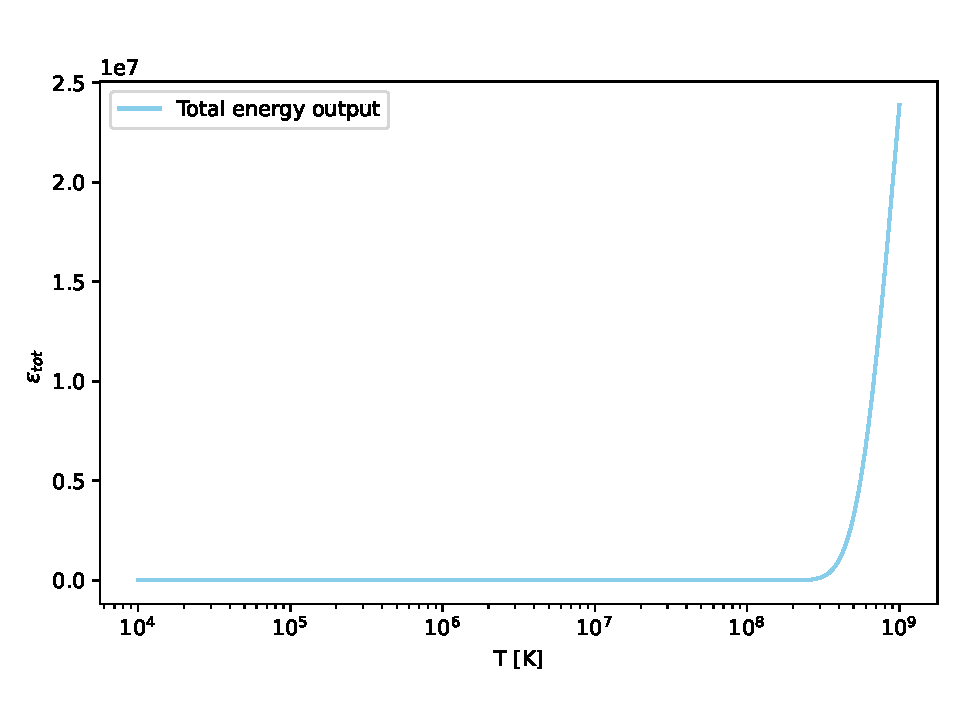
\includegraphics[width = 0.5\textwidth]{figures/energy_tot.pdf} 
    \caption{Total energy production as a function of the temperature of the stellar core.}
    \label{fig:tot}
\end{figure} 

\begin{figure*}
    \centering
    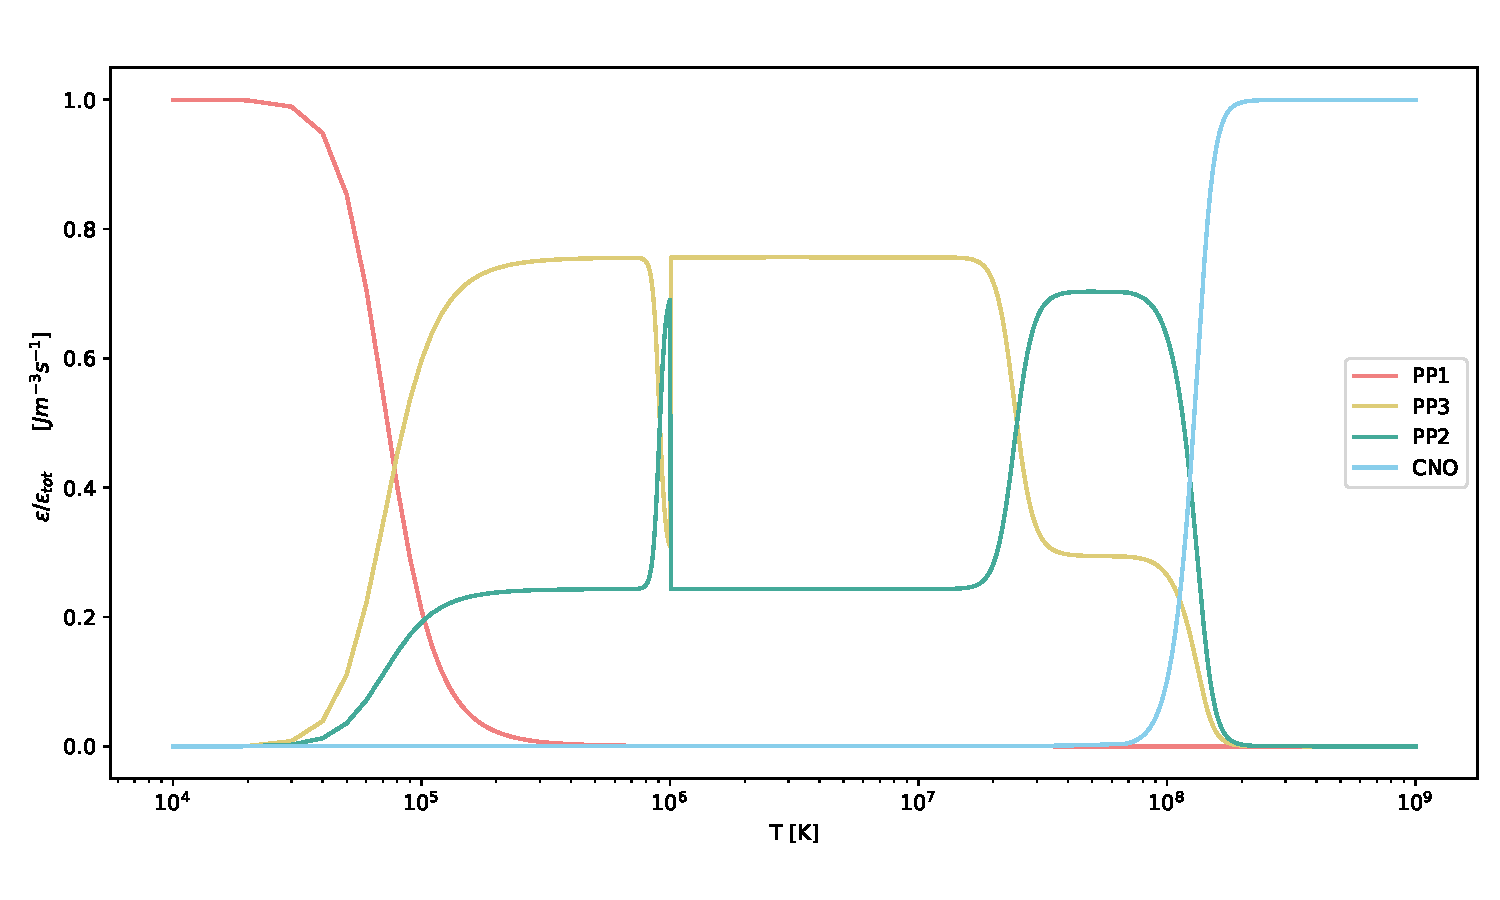
\includegraphics[width = 0.9\textwidth]{figures/energy.pdf} 
    \caption{Relative energy output of each fusion-reaction branch as a function of stellar-core-temperature, scaled by the total energy output. Calculated with an amount of $N=10^7$ steps of calculations.}
    \label{fig:enprod}
\end{figure*} 

\newpage
The Gamow peak for each relevant reaction of fusion is estimated by the Equation \eqref{eq:elmbd} for the produced energy $E\epsilon [10^{-17}, 10^{-13}]J$, normalized by each reactions maximum probability estimation is presented in Figure \ref{fig:prod}. Due to the scaling, the expression derived by Equation \eqref{eq:elmbd} in the estimations is reduced to the integral itself. 
\begin{figure}[H]
    \centering
    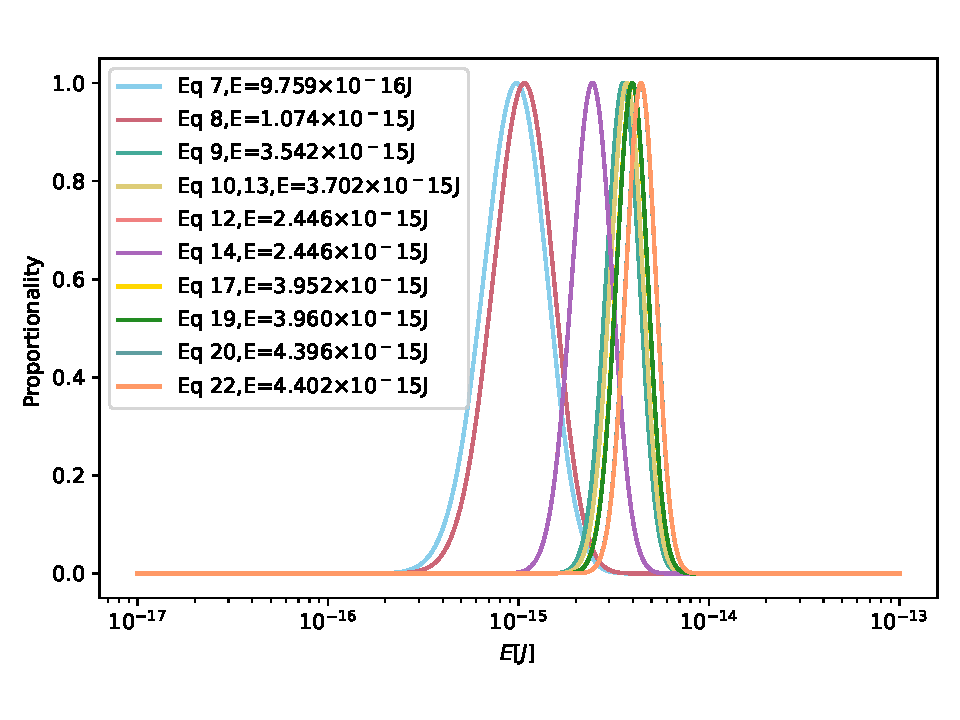
\includegraphics[width = 0.47\textwidth]{figures/peaks.pdf} 
    \caption{Gamow peaks for fusion reactions scaled by each maximum probability, related to the reaction equations presented in Section \ref{sec:theory}. Calculations estimated for $E\epsilon [10^{-17}, 10^{-13}]J$ with a logarithmic scale on the x-axis.}
    \label{fig:prod}
\end{figure} 

\section{Discussion}\label{sec:discussion}
From the sanity check ran for both temperatures $T=10^8$ and $T=1.57\times10^7K$, the overall relative error seems to keep below 0.001 while the temperature mimics that of the sun. In the case of the temperature $T=10^8$, it is clear that the accuracy of the model decreases to an accuracy below 0.004, which is not very significant. Noteworthy is the deviation for the sanity check equation 4, reaction described by Equation \eqref{eq:le7}, which increases all the way to 0.05 and fails the test for this instance. This entails an obvious error in either the reaction rate calculation, or somewhere within the energy output expression. The fault may also lay within the expression provided to the sanity check itself, though less likely. \\

The modelled energy lost due to neutrinos read in the Table \ref{tab:neu}, can be quality controlled by comparing them to the ones expected presented in Table \ref{tab:en}. As one can tell, due to the two iterations of Reaction \eqref{eq:r1} needed in order to produce the reactions in any of the fusion-reaction branches $2\times 0.265=0.530$,  the modelled results matches up with the expected values for each branch. \\
\newpage

The Figure \ref{fig:enprod} displays the energy production for each branch, and from it one can read a couple things about how this production takes place with an increasing temperature. When the temperature is within the interval $T\epsilon [0, \quad 10^{5}]$ the energy production is heavily dominated by the PP1-chain. In the interval $T \epsilon [10^5, \quad 10^{8}]$ the energy production is shared by the cycles PP2 and PP3, with a dominance by PP2 up until $T=10^{7.5}$. Once the temperature reaches $T=10^8$, the CNO cycle takes over the production, as expected from the theory presented in Section \ref{sec:theory}. The plots visualized in Figure \ref{fig:enprod} can sees in the light of \ref{fig:tot}, which visualizes the size of the scaling factor used to deduce the plots in Figure \ref{fig:enprod}. The graph shows an exponential growth in the energy production as the temperature of the core reaches about $10^8$, underlining the increase in energy output as a result of the CNO branch kicking in. Thereby one can conclude that the model for energy production is realistic. \\

The Figure \ref{fig:prod} visualizes the probability for certain reactions of fusion to occur at certain energy levels. The Figure shows a split between the probability peaks for the reactions described by Equation \eqref{eq:r1} and Equation \eqref{eq:rpp}, and the rest of the reactions - this indicates that the two reactions that are the base for all the rest of the reactions occurring within the stellar core is more likely to happen at a lower energy than the rest. The reactions that only happen in the CNO cycle requires a higher energy level in order for the probability of them occurring in the first place to peak.


\section{Conclusion}\label{sec:conclusion}
A model for a stellar engine, characterized by an energy production consisting of fusion of hydrogen into helium through the cycles \textbf{PP1}, \textbf{PP2}, \textbf{PP3} and \textbf{CNO} is developed. The accuracy of the model is evaluated through tests and analysis, and it is deemed to possess a sufficient level of accuracy. Inversely, the deviation in relative error presented by the sanity checks indicates a problem with the calculation of energy production by reaction described by Equation \eqref{eq:le7}. This deviation is noteworthy - however small it may seem - and is grounds for a conclusion of a dampened credibility. \\

The Figures \ref{fig:prod} and \ref{fig:enprod} depicts an energy production that can be derived from the theory presented in the section \ref{sec:theory}. This data analysis emphasizes the credibility of the model, in spite of the deviation detected by the sanity checks. We can conclude that the developed model simulates the energy production contributing to heating up the star in an adequate way, and is extensive enough to be used in further simulation of processes taking place within stars. \\



\section{Reflection}\label{sec:reflection}
This exercise has taught me a lot about the details of energy production within a stellar core. Through testing the code and comparing data to expected values for energy production, I was able to develop a model with an adequate level of accuracy. This was only achieved through a lot of trial and error, where I had to play close attention to units and function definitions in order to make it work. The operations needed to calculate the energy output was not necessarily that difficult to implement, as they were explained pretty well in the syllabus for the course \textit{AST3310: Astrophysical plasma and stellar interiors}, but the process helped gain a deeper understanding of said theory. I did not only gain a deeper understanding for how energy is produced in stars, but I also got a much needed refresher on how to program using python, and report writing using latex. 





\bibliographystyle{plain}
\bibliography{references}




\end{document}